%-----------------------------------------------------------------------------
%
%               Template for sigplanconf LaTeX Class
%
% Name:         sigplanconf-template.tex
%
% Purpose:      A template for sigplanconf.cls, which is a LaTeX 2e class
%               file for SIGPLAN conference proceedings.
%
% Guide:        Refer to "Author's Guide to the ACM SIGPLAN Class,"
%               sigplanconf-guide.pdf
%
% Author:       Paul C. Anagnostopoulos
%               Windfall Software
%               978 371-2316
%               paul@windfall.com
%
% Created:      15 February 2005
%
%-----------------------------------------------------------------------------


\documentclass[preprint]{sigplanconf}

% The following \documentclass options may be useful:

% preprint       Remove this option only once the paper is in final form.
%  9pt           Set paper in  9-point type (instead of default 10-point)
% 11pt           Set paper in 11-point type (instead of default 10-point).
% numbers        Produce numeric citations with natbib (instead of default author/year).
% authorversion  Prepare an author version, with appropriate copyright-space text.

\usepackage{amsmath}
\usepackage{graphicx}
\usepackage{hyperref}

\newcommand{\cL}{{\cal L}}

\begin{document}

\special{papersize=8.5in,11in}
\setlength{\pdfpageheight}{\paperheight}
\setlength{\pdfpagewidth}{\paperwidth}

\conferenceinfo{ICOOOLPS'17}{Month d--d, 20yy, City, ST, Country}
\copyrightyear{20yy}
\copyrightdata{978-1-nnnn-nnnn-n/yy/mm}\reprintprice{\$15.00}
\copyrightdoi{nnnnnnn.nnnnnnn}

% For compatibility with auto-generated ACM eRights management
% instructions, the following alternate commands are also supported.
%\CopyrightYear{2016}
%\conferenceinfo{CONF'yy,}{Month d--d, 20yy, City, ST, Country}
%\isbn{978-1-nnnn-nnnn-n/yy/mm}\acmPrice{\$15.00}
%\doi{http://dx.doi.org/10.1145/nnnnnnn.nnnnnnn}

% Uncomment the publication rights used.
%\setcopyright{acmcopyright}
\setcopyright{acmlicensed}  % default
%\setcopyright{rightsretained}

\titlebanner{Submitted for review to ICOOOLPS 2017}        % These are ignored unless
\preprintfooter{dart2java}   % 'preprint' option specified.

\title{{dart2java}: A Dart to Java Compiler}

\authorinfo{Andrew Krieger}{Univ. of California, Los Angeles}{akrieger@math.ucla.edu}
\authorinfo{Stanislav Manilov}{University of Edinburgh}{s.z.manilov@sms.ed.ac.uk}
\authorinfo{Matthias Springer}{Tokyo Institute of Technology}{matthias.springer@acm.org}

\maketitle

\begin{abstract}
We present the design and implementation of \emph{dart2java}, an experimental Dart to Java compiler. It is implemented in Dart on top of the new \emph{Kernel} intermediate representation and currently supports many but not all Dart language constructs. dart2java is a playground to evaluate performance implications of running Dart code on the JVM and to investigate if it is possible to write Dart code in a largely Java-dominated environment.

This paper describes the architecture of dart2java, performance optimizations such as non-nullability of primitive types and generic specialization (and their implicaitons), as well as ideas for language interoperability, i.e., calling Java code from Dart and vice versa.
\end{abstract}

% 2012 ACM Computing Classification System (CSS) concepts
% Generate at 'http://dl.acm.org/ccs/ccs.cfm'.
\begin{CCSXML}
<ccs2012>
<concept>
<concept_id>10011007.10011006.10011041.10011047</concept_id>
<concept_desc>Software and its engineering~Source code generation</concept_desc>
<concept_significance>500</concept_significance>
</concept>
</ccs2012>
\end{CCSXML}

\ccsdesc[500]{Software and its engineering~Source code generation}
% end generated code

% Legacy 1998 ACM Computing Classification System categories are also
% supported, but not recommended.
%\category{CR-number}{subcategory}{third-level}[fourth-level]
%\category{D.3.0}{Programming Languages}{General}
%\category{F.3.2}{Logics and Meanings of Programs}{Semantics of Programming Languages}[Program analysis]

\keywords
Dart, Java, compiler, source code generation

\section{Introduction}
Dart is an object-oriented class-based programming language developed by Google and was originally designed as a replacement of JavaScript in the Dartium web browser, which was capable of directly executing Dart code. Nowadays, Dart can be used for writing standalone applications running in the \emph{Dart VM} and for writing web applications using a source-to-source compiler to JavaScript. This paper presents the design and implementation of dart2java, an experimental Dart to Java compiler. Its design is inspired by Google's Dart to JavaScript compiler and reuses some of their ideas (such as the ``patching'' mechanism described later). 

At first sight, Dart's syntax is similar to Java but it provides special notations for commonly used features such as list/map literals, getter/setter methods or factory constructors. Therefore, we think that Dart is an interesting alternative for Java programmers. The motivation for dart2java is twofold: First, dart2java provides a migration from a most Java-dominated environment to a Dart environment, because Java code can be called from Dart (and vice versa). Second, dart2java is experiment to see if Dart code is suitable to be executed on the JVM. Third, dart2java allows programmers to write Dart code for platforms where only Java is available.


\section{Architecture}
Every Dart system has two main components: A Dart implementation (compiler/interpreter; e.g., the Dart VM or dart2java) and the Dart SDK. The latter one contains Dart source code of core interfaces (such as \texttt{int} and \texttt{object}) and standard library classes, and is meant to be shared by all Dart implementations. The Dart SDK provides two kinds of variation points for Dart implementations: First, some methods are declared as external, i.e., it is up to the Dart implementation to provide an implementation for the method. Second, certain core classes are pure interfaces (all methods are abstract) and it is up to the Dart implementation to provide an implementation class; only the public SDK interface type will be exposed to the programmer.

\subsection{Compiling User Programs}
\begin{figure}[!htp]
    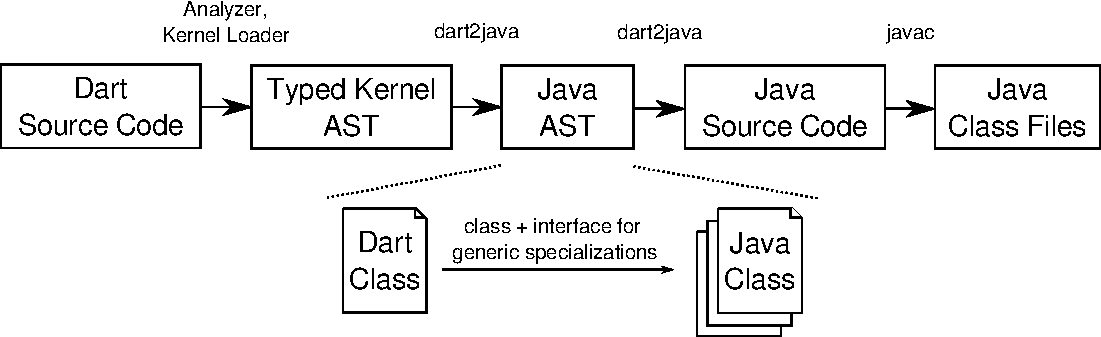
\includegraphics[width=\columnwidth]{dart2java_compile_user_code.pdf}
    \label{fig:user_code_compilation}
    \caption{User Code Compilation Process}
\end{figure}
Figure~\ref{fig:user_code_compilation} shows the compilation process for Dart programs. dart2java uses \emph{Analyzer} and \emph{Kernel}\footnote{\url{https://github.com/dart-lang/kernel}} to generate a generated a typed abstract syntax tree of every Dart class. This Dart AST is then transformed into a Java AST, generating one Java interface and one Java class for every Dart class, along with generic specializations for generic classes (see Section~\ref{sec:generic_spec}). The Java interface is necessary because every Dart class implicitly defines an interface that can be implemented by any class. The resulting Java classes can then be compiled and run with a copy of the compiled Dart SDK in the classpath.

\subsection{Compiling the Dart SDK}
The compilation process for the Dart SDK is mostly identical but starts with \emph{patching}: Some external methods are replaced with pure Dart implementations in dart2java. For example, the external factory constructor\footnote{A factory constructor is a static method that is run when instantiating a class. It may return an instance of a subclass.} for \texttt{Map} is replaced with a concrete factory constructor creating an instance of \texttt{LinkedHashMap}, a class that is implemented in Dart and shipped together with dart2java. Patching allows us to implement external methods in Dart without having to change the Dart SDK itself.


\section{Performance: Primitive Types Only}

\subsection{Primitive Types Only}

\subsection{Non-nullability}

\subsection{Generic Specialization}
\label{sec:generic_spec}

\subsection{Benchmarks}


\section{Language Interoperability}

\subsection{Java Components in Dart}

\subsection{Dart Components in Java}


\section{Related Work}
Generic specialization in .NET using JIT, language interoperability in related projects


\section{Conclusion}
Preliminary findings, can the same techniques be applied to other projects?

\acks
Thank Vijay, Jennifer, Leaf

% The 'abbrvnat' bibliography style is recommended.

\bibliographystyle{abbrvnat}

% The bibliography should be embedded for final submission.

\begin{thebibliography}{}
\softraggedright

\bibitem[Smith et~al.(2009)Smith, Jones]{smith02}
P. Q. Smith, and X. Y. Jones. ...reference text...

\end{thebibliography}


\end{document}
